\subsection{Altura do feixe}\label{sec:5.6}
No cálculo da largura do feixe, assumiu-se que a emissão quântica não alterava a direção do movimento do elétron. Esta suposição não está totalmente correta. Qualquer evento quântico individual pode causar um pequeno impulso transversal no elétron. Pode-se pensar que um evento quântico corresponde à emissão de um fóton com momento $u/c$ com ângulo $\theta_\gamma$ com relação ao momento do elétron. Assim, haverá uma componente transversal de momento igual a $\theta_\gamma u/c$. A conservação de momento requer que haja uma mudança correspondente no momento transversal $x' E_0/c$ -- veja a \autoref{fig:fig45}. Isto é, haverá uma mudança em $x'$ dada por
\begin{align}
	\delta x' = \frac{u}{E_0} \theta_x\label{eq:5.98}
\end{align}
onde $\theta_x$ é a projeção horizontal de $\theta_\gamma$. A maior parte da radiação síncrotron é emitida na direção do movimento do elétron, mas é espalhada em um cone com ângulo médio $1/\gamma$. Então pode-se considerar que $\theta_\gamma$ é tipicamente da ordem de $1/\gamma$. O termo $\eta'$ que aparece na equação \eqref{eq:5.67} tem sua ordem de magnitude próxima da unidade, então negligenciar a contribuição da equação \eqref{eq:5.98} no movimento radial é razoável.

\begin{figure}[!htb]
	\centering
	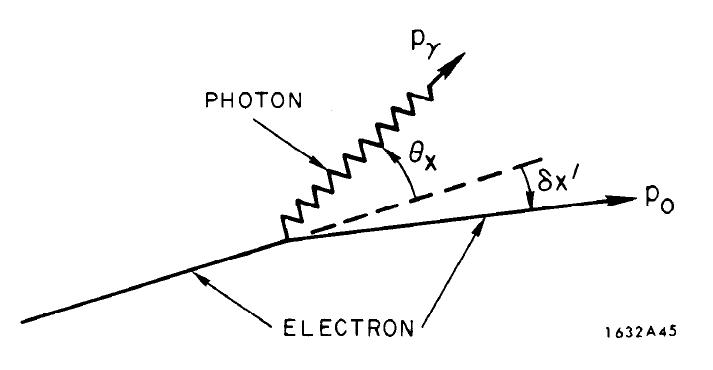
\includegraphics[width=0.9\linewidth]{./Figuras/fig45.jpeg}
	\caption{Mudança na direção do movimento do elétron devido à emissão de um fóton. Retirado de \cite{sands1970physics}.}
	\label{fig:fig45}
\end{figure}

No entanto, deve-se considerar quais serão os efeitos causados pela emissão quântica no movimento betatron vertical. Se a órbita ideal está apenas sobre o plano, não existem efeitos de primeira ordem advindos da emissão quântica no movimento vertical (isto é, a função vertical correspondente é praticamente nula). O único efeito remanescente seria advindo da distribuição angular da radiação. Hora de analisar a magnitude deste efeito.

Pode-se utilizar os resultados da análise anterior substituindo a equação \eqref{eq:5.67} por
\begin{align}
	\delta z = 0\ \ \ \ \ \ \ \delta z' = \frac{u}{E_0}\theta_z
\end{align}
onde $\theta_z$ é a projeção vertical do ângulo de emissão de um fóton. A equação \eqref{eq:5.73} se tornaria -- lembrando que o subscrito $z$ serve apenas para lembrar que uma oscilação vertical está sob análise --
\begin{align}
	\delta \mean{a_z^2} = \frac{u^2}{E_0^2} \theta_z^2 \beta_z(s_2)
\end{align}
Seguindo com as derivações, no lugar da equação \eqref{eq:5.81} seria
\begin{align}
	\sigma_{z}(s) = \frac{1}{4} \tau_z Q_z \beta_z(s)
\end{align}
com
\begin{align}
	Q_z = \frac{\mean{\mathscr{N}\mean{u^2 \theta_z^2}\beta_z}_s}{E_0^2}
\end{align}
Para avaliar $Q_z$, é preciso levar em consideração a variação do espectro de frequência da radiação síncrotron com o ângulo de emissão. Como o efeito analisado é sempre pequeno, um cálculo aproximado é suficiente. Suponha, primeiramente, a aproximação
\begin{align}
	\mean{u^2 \theta_z^2} \approx \mean{u^2}\mean{\theta_z^2}
\end{align}
Pode-se aproximar a média do quadrado da projeção angular por $1/2$ vezes o valor médio de $\theta_\gamma$, ou seja,
\begin{align}
	\mean{\theta_z^2} \approx \frac{1}{2 \gamma_0^2}
\end{align}
Também aproxima-se $\beta_z(s)$ pelo seu valor típico $\beta_n$. Então, tem-se que
\begin{align}
	Q_z \approx \frac{\mean{\mathscr{N}\mean{u^2}}_s \beta_n}{\gamma_0^2 E_0}
\end{align}
Lembre-se que a média de $\mathscr{N}\mean{u^2}$ é apenas $Q_\epsilon$ definido na \autoref{sec:5.2}. Logo,
\begin{align}
	\frac{\sigma_z^2}{\sigma_\epsilon^2} \approx \frac{\tau_z Q_z \beta_n}{\tau_\epsilon Q_\epsilon} \approx \frac{J_\epsilon}{J_z}\frac{\beta_n^2}{\gamma_0^2 E_0^2}
\end{align}
Para uma órbita ideal plana, $J_z \approx 1$. Considerando apenas o caso isomagnético, pode-se tomar $\sigma_\epsilon^2/E_0^2$ da equação \eqref{eq:5.48} e escrever que
\begin{align}
	\sigma_z^2 \approx \frac{C_q \beta_n^2}{\rho_0}\ \ (isomag.)\label{eq:5.107}
\end{align}
Grosseiramente falando, $\beta_n$ é da mesma ordem que $\rho_0$ e
\begin{align}
	\sigma_z^2 \approx C_q \beta_n
\end{align}
As oscilações verticais induzidas pela emissão quânticas são independentes da energia e menores que as oscilações radiais por um fator $1/\gamma_0^2$. De fato, elas são muito pequenas.

As oscilações verticais dadas pela equação \eqref{eq:5.107} são tão pequenas que elas sempre serão desprezíveis em comparação com as oscilações verticais produzidas por qualquer outro efeito maior -- um acoplamento da oscilação de energia advinda das oscilações betatron horizontais nas oscilações verticais. Estes efeitos não foram considerados na análise da natureza das oscilações betatron (\autoref{part2}) pois estas perturbações são essencialmente de segunda ordem. Uma análise das perturbações esperadas devido a imperfeições na construção de um anel de armazenamento real mostra que o acoplamento entre as oscilações horizontal e vertical tende a produzir uma altura de feixe a qual é ao menos uma pequena porcentagem da largura do feixe, a qual tem um valor muito maior que a largura mínima intrínseca calculada.

De fato, como será visto depois, às vezes deseja-se obter uma altura de feixe maior que a produzida pelas imperfeições acidentais. E isto pode ser feito introduzindo propositalmente um acoplamento entre as oscilações vertical e horizontal -- que pode ser causado por elementos magnéticos especiais (quadrupolos \textit{skew}) ou operando o anel próximo da ressonância entre $\nu_x$ e $\nu_z$, ou pela combinação destas duas maneiras.

Uma análise detalhada do acoplamento das oscilações horizontal e vertical não faz parte do escopo deste documento, mas uma visão fenomenológica do assunto seria interessante. Suponha que $g_x$ e $g_z$ representem o quadrado dos invariantes das amplitudes das oscilações radial e vertical, respectivamente. Isto é,
\begin{align}
	g_x = \frac{\sigma_x^2(s)}{\beta_x(s)}\ \ \ \ \ \ \ g_z = \frac{\sigma_z^2(s)}{\beta_z(s)}\label{eq:5.109}
\end{align}
Para o caso especial em que as taxas de amortecimento das oscilações vertical e horizontal são iguais, pode-se argumentar da seguinte forma. Sem acoplamento
\begin{align}
	g_x = g_0 = \frac{1}{4} \tau_x Q_x
\end{align}
-- da equação \eqref{eq:5.81}. Quando o acoplamento é considerado, a excitação quântica das oscilações radiais pode ser dividida com as oscilações verticais em qualquer proporção numa divisão igualitária. Isto é, tem-se
\begin{align}
	g_z = \kappa g_x
\end{align}
onde $\kappa$ é o "coeficiente de acoplamento". A princípio, $\kappa$ pode ser qualquer número entre 0 e 1, apesar de na prática ser geralmente difícil reduzir $\kappa$ abaixo de 1 por cento ou algo em torno disso. Como a excitação está sendo compartilhada, as excitações combinadas precisam ser iguais a $g_0$:
\begin{align}
	g_x + g_z = g_0
\end{align}
De forma equivalente,
\begin{align}
	g_z = \frac{\kappa}{1+\kappa}g_0\\
	g_x = \frac{1}{1+\kappa}g_0
\end{align}

A excitação $g_0$ pode ser avaliada a partir de qualquer expressão derivada para $\sigma_{x\beta}^2$ (sem considerar acoplamento) na \autopageref{sec:5.6}. Para qualquer coeficiente de acoplamento $\kappa$, $g_x$ e $g-z$ são obtidos; e a partir da largura e da altura médias do feixe, $\sigma_x$ e $\sigma_z$ podem ser encontrados pela equação \eqref{eq:5.109}.

Desta forma, a altura máxima do feixe pode ser obtida quando $\kappa=1$. Então $(g_z)_{max} = g_0/2$ e
\begin{align}
	\frac{(\sigma_z^2)_{max}}{\beta_z} = \frac{1}{8} \tau_x Q_x
\end{align}
Usando os resultados aproximados analisados anteriormente para um campo guia isomagnético, pode-se escrever que o \textit{spread} máximo vertical do feixe é
\begin{align}
	\frac{(\sigma_z^2)_{max}}{\beta} \approx \frac{C_q \alpha R \gamma_0^2}{2 \rho_0 \nu_x}\ \ (isomag.)
\end{align}
onde, como foi assumido que $\tau_x = \tau_z$, $J_x = J_z = 1$.

Em princípio, tanto a largura quanto a altura do feixe não podem ser aumentados por estimulação artificial das oscilações transversais -- por exemplo, por aplicação periódica de impulsos elétricos ou forças magnéticas sobre o feixe armazenado. Na prática, no entanto, estes estímulos externos irão resultar em movimentos coerentes de grandes quantidades de elétrons em um \textit{bunch}, o que sabe-se que causa efeitos depreciativos na luminosidade de feixes colisores. Apesar disso, é pouco provável que o aumento do feixe possa ser usado em anéis mais modernos que possam operar com diferentes sintonias para cada feixe colisor.